\documentclass[a4paper, 11pt]{article}
\usepackage[utf8]{inputenc} % Change according your file encoding
\usepackage{float}
\usepackage{graphicx}
\usepackage{url}
\usepackage{listings}

%opening
\title{Seminar Report: Opty}
\author{Erkki Heino, Bastien Scanu}
\date{\today{}}

\begin{document}

\maketitle

\section{Introduction}
This session consists in the implementation of a transaction server using optimistic concurrency control.


\section{Work done}
For the basic program, we just had to fill the gaps so we didn't have to take major design decisions. We took some decisions when we modified the files to do the experiments.\\
To modify the Read/Write ratio, we modified the do\_transactions function, replacing the write and the read by twxo functions \emph{do\_reads} and \emph{do\_writes}:
\lstset{language=erlang}   
\begin{lstlisting}
do_reads(_, _, _, 0) ->
    ok;

do_reads(Handler, Refx, Num, N) ->
    Handler ! {read, Ref, Num},
    do_reads(Handler, Ref, Num, N-1).

do_writes(_, _, _, 0) ->
    ok;

do_writes(Handler, Num, Value, N) ->
    Handler ! {write, Num, Value+1},
    do_writes(Handler, Num, Value+1, N-1).

\end{lstlisting}
The number of reads and writes to do during one transaction were implemented as parameters of the \emph{opty:start} function.\\ \\ 

To generate randomly a subset of n entries, we created a dedicated function in the opty module.
\begin{lstlisting}
generate_subset(0, _, Subset) ->
    list_to_tuple(Subset);

generate_subset(Number, Entries, Subset) ->
    Temp = random:uniform(Entries),
    case lists:any(fun(E) -> E == Temp end, Subset) of
	true ->
	    generate_subset(Number, Entries, Subset);
	false ->
	    generate_subset(Number - 1, Entries, [Temp|Subset])
    end.
\end{lstlisting}

We call this function when we create a client, and then the subset will be transmitted as a parameter to the client. When a client chooses which entry it will access, it can only access one of the entries of the subset thanks to these two lines of code:
\begin{lstlisting}
Index = random:uniform(tuple_size(Subset)),
Num = element(Index, Subset),
\end{lstlisting}

\section{Experiments}

\subsection{Number of clients}
In this experiment, we will study the influence of the number of clients on the success rate of transactions. We will set the number of entries to 10, the number of updates per transaction to 4 and the time to ten seconds. We did the experiment for 1 to 11 clients.

\begin{figure}[H]
\begin{center}
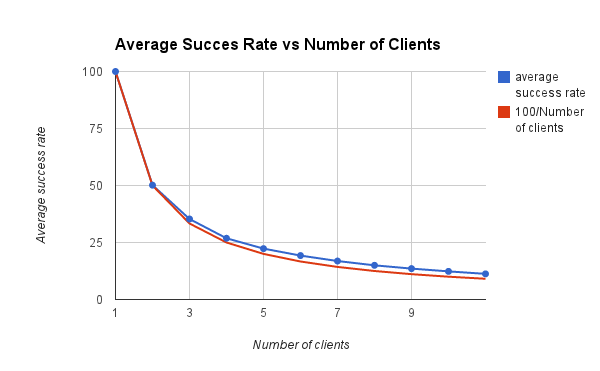
\includegraphics[scale=0.5]{exp1.png}
\caption{Impact of the number of clients on the average success rate}
\end{center}
\end{figure}

\subsubsection{Open Question}
As we see in the figure, the average success rate of transactions decreases when the number of clients increases. Moreover, this success rate seems to be close to 100/number of clients. We also observe that the success rate is the same for all the clients (less than 1\% of difference in all the cases).


\subsection{Number of entries}
In this experiment, we will study the influence of the number of entries on the success rate of transactions. We will set the number of clients to 10, the number of updates per transaction to 4 and the time to ten seconds. We did the experiment for 1 to 11 entries, and two others measurements for 20 and 50, just in order to see if there is a more significant evolution with bigger numbers.

\begin{figure}[H]
\begin{center}
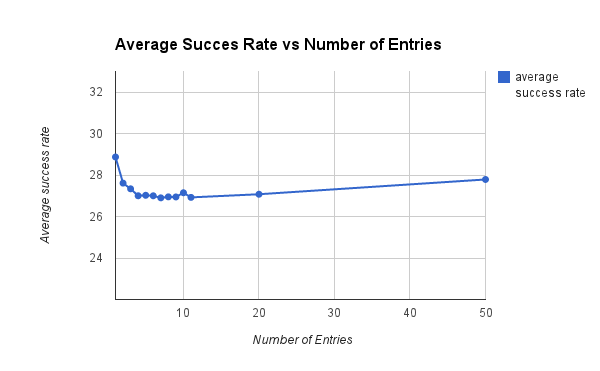
\includegraphics[scale=0.5]{exp2.png}
\caption{Impact of the number of entries on the average success rate}
\end{center}
\end{figure}

\subsubsection{Open Question}
As we see in the figure, there is no clear correlation between the number of entries and the succes rate of transactions. The only thing that we can say is that the rate is a bit higher when there is only one entry (around 29\%, against 27\% for other values, the experiment was repeated several times with the same result). We also observe that the success rate is the same for all the clients (less than 1\% of difference in all the cases).


\subsection{Number of updates}
In this experiment, we will study the influence of the number of updates on the success rate of transactions. We will set the number of clients to 4, the number of entries to 10 and the time to ten seconds. We did the experiment for 1 to 11 updates, and one other measurement for 50, just in order to see if there is a more significant evolution with bigger numbers.

\begin{figure}[H]
\begin{center}
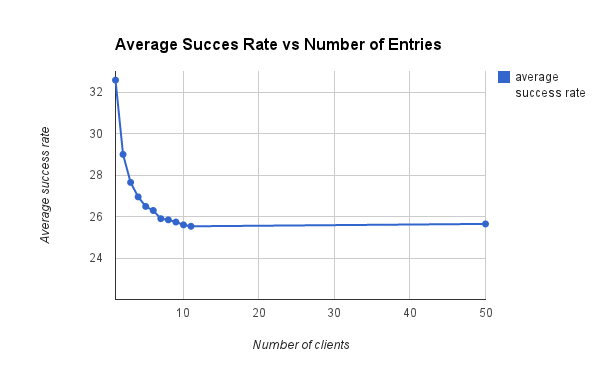
\includegraphics[scale=0.5]{exp3.png}
\caption{Impact of the number of updates on the average success rate}
\end{center}
\end{figure}

\subsubsection{Open Question}
As we see in the figure, the average success rate of transactions decreases when the number of clients increases, from 32,5\% for 1 update to 25,5\% for ten. For numbers bigger than ten entries, the evolution is negligible. We also observe that the success rate is the same for all the clients (less than 1\% of difference in all the cases).


\subsection{Ratio of read and write operations per transaction}
In this experiment, we will study the influence of ratio of read and write operations per transaction on the success rate of transactions. We will set the number of clients to 4, the number of entries to 10, the number of updates to 4 and the time to ten seconds. We did the experiment for different ratios: when there is only one kind of operation performed, and for ratios of 2, 3, 4, 5 and 10.

\begin{figure}[H]
\begin{center}
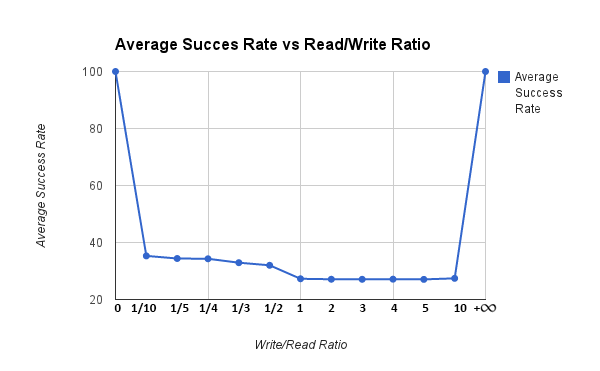
\includegraphics[scale=0.5]{exp4.png}
\caption{Impact of the read/write ratio on the average success rate}
\end{center}
\end{figure}

\subsubsection{Open Question}
We can see on Figure4 that the uncommited transactions are the result of the concurrency between read and write operations. Indeed, when we perform only reads or only writes, we can see that all transactions are commited. We also not that when we have a number of writes superior or equal to the number of reads (and if there is at least one read operation), we always have the same average success rate for any ratio. Finally, when we have more reads than writes, the average succes rate increases when the ration increases.

\subsection{Percentage of accessed entries}
In this experiment, we will study the influence of the percentage of accessed entries on the success rate of transactions. We will set the number of clients to 4, the number of entries to 10, the number of updates to 4 and the time to ten seconds. We tried the experiment with values from 10\% until 100\%.

\begin{figure}[H]
\begin{center}
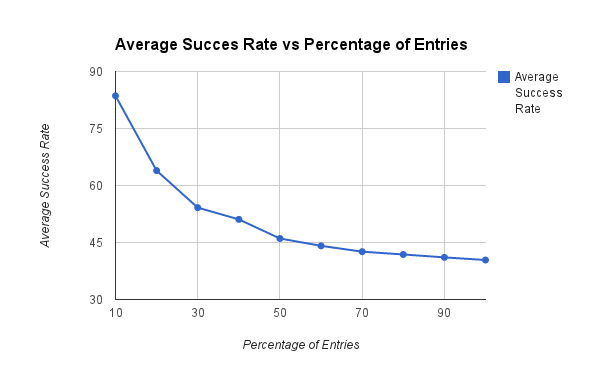
\includegraphics[scale=0.5]{exp5.png}
\caption{Impact of the percentage of accessed entries on the average success rate}
\end{center}
\end{figure}

\subsubsection{Open Question}
As we could expect, we see that the success rate decreases when the percentage of accessed entries increases, because the risk of conflicts is higher. The success rate is different for each client and depends on the different subset of entries accessed by all the clients. If a client has in its subset only entries that other clients cannot access, its success rate will be 100\%, but the more entries it has to share with other clients, the more its success rate will decrease. The success rate highly depends on the random generation of the subset, so we repeated each experiment ten times and took the average value to have something meaningful.


\subsection{Split the opty module}

\subsubsection{Open Question}

\section{Personal opinion}
This activity seems to be a logical continuation of the Paxy seminar. The program is more complete and also very interesting, and the experiments allowed us to understand better how the algorithm works.

\end{document}
